% !TeX root = holoclean.tex
% !TeX encoding = UTF-8
% !TeX spellcheck = en_US

\section{Data Repairing}\label{sec:introduction}
  Data is a central aspect in most enterprises.
  It is the basis for operational and strategic business decision making.
  However, real world data is flawed and contains errors, which can impair reporting, customer service, and production facilitation.
  Studies show that poor data quality leads to costs of billions of dollars~\cite{Redman:quality_disaster, cost_of_low_qual}.
  Maintaining the quality and consistency of business data has therefore become a critical task.

  \subsection{Data cleaning}
  One way to improve data quality is data cleaning.
  It consists of two steps: Error detection and data repairing.
  Error detection describes the process of identifying incorrect values in a dataset.
  Subsequently data repairing transforms the erroneous dataset into a new one removing detected errors, so the new dataset adheres to data quality requirements.

  \subsection{Related work}
  Many researchers have made efforts to automate the task of error detection.
  \begin{itemize}
    \item \textbf{TODO:}
    \item Most of the approaches try to detect the violation of \glspl{ic}.
    \item duplicate detection
    \item outlier detection
  \end{itemize}

  Data repairing techniques can be classified according to whether and how humans are involved in the repairing process.
  On the one end there are fully automatic approaches, such as SCARE~\cite{scare}, that leverage machine learning and intelligent partition algorithms to repair a database without the need of user input.
  On the other end there are data wrangling tools that make extensive use of human knowledge to clean a dirty dataset.
  For example, Data Wrangler~\cite{data_wrangler}, the successor of Potter's Wheel~\cite{potters_wheel}, provides a visual interface for cleaning a dataset.
  Based on data statistics it creates visual suggestions for data transformations.
  The user selects and executes those transformations to create a cleaned dataset instance.
  The tool can export the transformation sequence, to repeat the process on another dataset.
  This makes it an appropriate tool for the manual definition of ETL processes.
  The final version of the tool, Trifacta Wrangler~\cite{trifacta_wrangler}, is developed commercially.

  All those tools~\cite{scare,potters_wheel,data_wrangler,trifacta_wrangler} use quantitative statistics of the dataset itself to repair errors in it.
  Besides that, state-of-the-art methods also use \glspl{ic}~\cite{ajax,gdr,editing_rules,data_tamer} and external knowledge~\cite{katara}, such as dictionaries, knowledge bases, or domain expert annotations, as input signals.
  Figure~\ref{fig:tools} shows those tools aligned on their level of user interaction needed to perform data repairing and the usage of the three different input signals.

  \begin{figure*}
    \centering
    % !TeX root = tools.tex
% !TeX encoding = UTF-8
% !TeX spellcheck = en_US

\documentclass[crop,tikz]{standalone}
\usetikzlibrary{
  positioning,
  arrows
}

\makeatletter
\@ifundefined{holoclean}{%
  \newcommand{\holoclean}{HoloClean}%
}{}
\makeatother

\begin{document}

% Data Repairing Tools Diagram
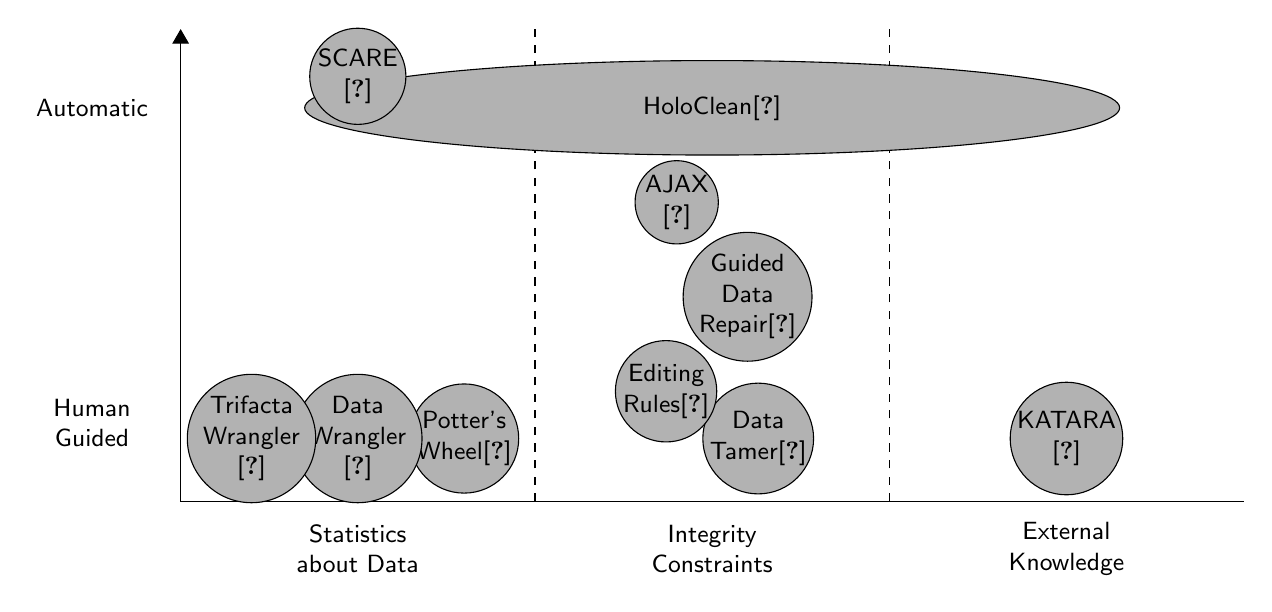
\begin{tikzpicture}[
    xscale=4.5, yscale=4,>=triangle 60,font=\sffamily,
    tool/.style={
      circle,
      draw=black,
      fill=black!30,
      inner sep=0pt,
      minimum size=25pt
    }
  ]
  \small  
  
  \begin{scope}
    \draw[black,] (-1.5,-0.25) -- (1.5,-0.25) ;
    \draw[black,->] (-1.5,-0.25) -- (-1.5,1.25) ;
    \draw[black,dashed] (-0.5,-0.25) -- (-0.5,1.25) ;
    \draw[black,dashed] (0.5,-0.25) -- (0.5,1.25) ;
    
    \draw[tool] (0,1) ellipse (1.15 and 0.15) node {\holoclean{}\cite{holoclean}};
    
    \node[tool, align=center] at (1,-0.05) {KATARA\\\cite{katara}};
    
    \node[tool, align=center] at (0.13,-0.05) {Data\\Tamer\cite{data_tamer}};
    \node[tool, align=center] at (-0.13,0.1) {Editing\\Rules\cite{editing_rules}};
    \node[tool, align=center] at (0.1,0.4) {Guided\\Data\\Repair\cite{gdr}};
    \node[tool, align=center] at (-0.1,0.7) {AJAX\\\cite{ajax}};
    
    \node[tool, align=center] at (-0.7,-0.05) {Potter's\\Wheel\cite{potters_wheel}};
    \node[tool, align=center] at (-1,-0.05) {Data\\Wrangler\\\cite{data_wrangler}};
    \node[tool, align=center] at (-1.3,-0.05) {Trifacta\\Wrangler\\\cite{trifacta_wrangler}};
    
    \node[tool, align=center] at (-1,1.1) {SCARE\\\cite{scare}};
    
    \node[align=center] at (-1.75,1) {Automatic};
    \node[align=center] at (-1.75,0) {Human\\Guided};
    
    \node[align=center] at (1,-0.4) {External\\Knowledge};
    \node[align=center] at (0,-0.4) {Integrity\\Constraints};
    \node[align=center] at (-1,-0.4) {Statistics\\about Data};
  
  \end{scope}
\end{tikzpicture}

\end{document}
    %% !TeX root = ../holoclean.tex
% !TeX encoding = UTF-8
% !TeX spellcheck = en_US

% Data Repairing Tools Diagram
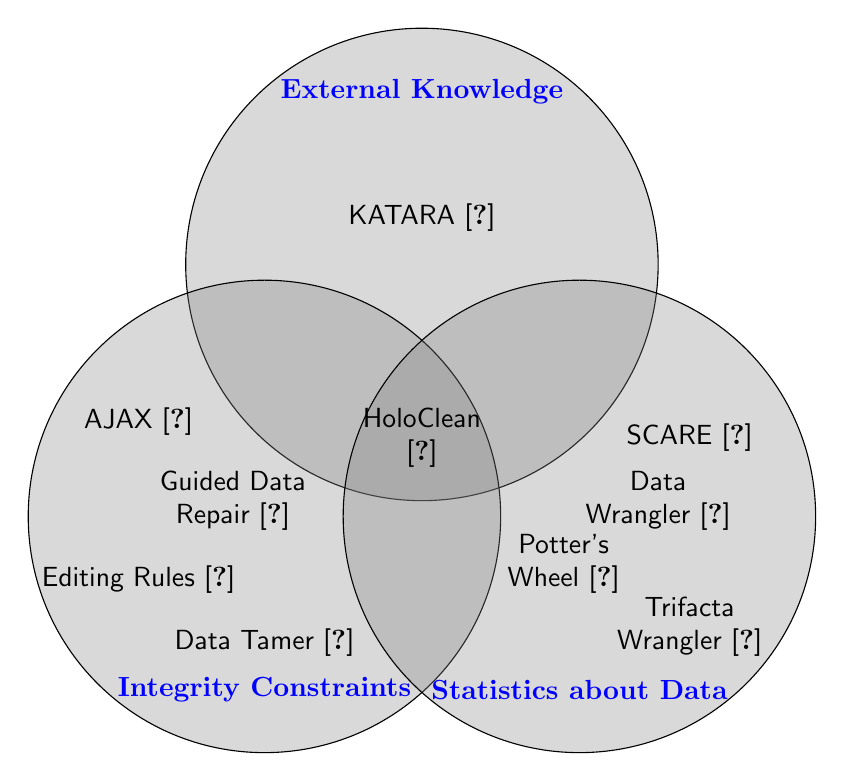
\begin{tikzpicture}[
    xscale=4, yscale=4,>=triangle 60,font=\sffamily,
    tool/.style={
      circle,
      align=center
    },
    bubble/.style={
      draw=black,
      fill=black!50,
      fill opacity=0.3
    }
  ]  
  
  \begin{scope} 
    
    % Venn bubbles
    \draw[bubble] (0,0.55) circle (0.75);
    \node[font=\bfseries, text=blue] at (0,1.1) {External Knowledge};
    
    \draw[bubble] (-0.5,-0.25) circle (0.75);
    \node[font=\bfseries, text=blue] at (-0.5,-0.8) {Integrity Constraints};
    
    \draw[bubble] (0.5,-0.25) circle (0.75);
    \node[font=\bfseries, text=blue] at (0.5,-0.8) {Statistics about Data};
    
    % Middle
    \node[tool] at (0,0) {\holoclean{}\\\cite{holoclean}};
    
    % Up
    \node[tool] at (0,0.7) {KATARA \cite{katara}};
    
    % Left
    \node[tool] at (-0.9,0.05) {AJAX \cite{ajax}};
    \node[tool] at (-0.6,-0.2) {Guided Data\\Repair \cite{gdr}};
    \node[tool] at (-0.9,-0.45) {Editing Rules \cite{editing_rules}};
    \node[tool] at (-0.5,-0.65) {Data Tamer \cite{data_tamer}};
    
    % Right
    \node[tool, align=center] at (0.85,0) {SCARE \cite{scare}}; 
    \node[tool, align=center] at (0.45,-0.4) {Potter's\\Wheel \cite{potters_wheel}};
    \node[tool, align=center] at (0.75,-0.2) {Data\\Wrangler \cite{data_wrangler}};
    \node[tool, align=center] at (0.85,-0.6) {Trifacta\\Wrangler \cite{trifacta_wrangler}};
    
  \end{scope}
  
\end{tikzpicture}
    \caption{Data Repairing Tools in Context}
    \label{fig:tools}
  \end{figure*}

  %% !TeX root = holoclean.tex
% !TeX encoding = UTF-8
% !TeX spellcheck = en_US

\begin{table*}
    \caption{Data Repairing Tool Matrix}
    \label{tab:tools}
    \newcommand{\h}{High}
    \newcommand{\m}{Medium}
    \newcommand{\lo}{Low}
    \begin{tabular}{lcccc}
    \toprule
    	\textbf{Repairing Tool}                    & \textbf{Degree of}  &          \multicolumn{3}{c}{\textbf{Input Signals}}          \\
    	                                           & \textbf{Automation} & \textbf{Statistics} & \textbf{ICs} & \textbf{Ext. Knowledge} \\
    \midrule
    	\holoclean{} \cite{holoclean}              &         \h          &          X          &      X       &            X            \\
    	SCARE \cite{scare}                         &         \h          &          X          &              &  \\
    	AJAX \cite{ajax}                           &         \h          &                     &      X       &  \\
    	Guided Data Repair \cite{gdr}              &         \m          &                     &      X       &  \\
    	Editing Rules \cite{editing_rules}         &         \m          &                     &      X       &  \\
    	Data Tamer \cite{data_tamer}               &         \lo         &                     &      X       &  \\
    	KATARA \cite{katara}                       &         \lo         &                     &              &            X            \\
    	Potter's Wheel \cite{potters_wheel}        &         \lo         &          X          &              &  \\
    	Data Wrangler \cite{data_wrangler}         &         \lo         &          X          &              &  \\
    	Trifacta Wrangler \cite{trifacta_wrangler} &         \lo         &          X          &              &  \\
    \bottomrule
    \end{tabular}
  \end{table*}

  \subsection{Introducing \holoclean{}}
  Most of the tools limit themselves to only one signal to perform data repairing, ignoring other information sources.
  Each type of signal is associated with a different action on the dataset and has its own downsides.
  Data repairs that use \glspl{ic} could introduce incorrect repairs, because they are relying on the \textit{minimality principle} and assume that most of the data values are clean.
  This is not necessarily the case and minimal repairs not always correspond to correct repairs~\cite{holoclean}.
  Repair algorithms relying on external information are dependent on the coverage of the external data source and can therefore perform poorly.
  Quantitative statistics heavily depend on the available information in the dataset itself.
  For small datasets and unfortunate situations this can drastically decrease repairing quality.
  
  \citeauthor{holoclean} therefore propose a holistic data repairing approach that includes all aforementioned signals into one framework: \holoclean{}~\cite{holoclean}.
  To tackle the problem that different signals could suggest conflicting repairs they convert all signals into features of a probabilistic model.
  Based on this combined view on the data and their inconsistencies they can then use statistical learning and probabilistic inference to suggest repairs for the dataset.
  
  \subsection{Overview}
  \begin{itemize}
    \item following work, we explain \holoclean{} in more detail
    \item describe chapters
  \end{itemize}


\section{Background}\label{sec:background}
  In the following paragraphs we review the terminology used in the next sections.
  
  \subsection{Integrity constraints}
  Users of the \holoclean{} framework can specify \glspl{ic} in form of denial constraints, which combine different types of integrity definitions.
  Functional Dependencies as well as conditional functional dependencies can be expressed as denial constraints~\cite{fd_to_dc}.
  A denial constraint states that all predicates of it cannot be true at the same time, otherwise, there is a consistency conflict.
  It is notated as $\forall t_i, t_j \in D: \neg(P_1 \wedge \dots \wedge P_K)$.
  Over all tuples $t \in D$ of a database instance $D$ not all predicates $P_k$ are allowed to be true.
  $P_k$ are defined as $v_1 \circ v_2$ or $v_1 \circ c$ with $v_1, v_2 \in \{t_i.A, t_j.A\}$, where $A$ denotes an attribute of the dataset $D$.
  The operator $\circ$ can be one of $\{=,<,>,\neq,\leq,\geq\}$~\cite{chu2013discoveringdc}.
  For readability reasons we use functional dependencies of the form $A_1 \to A_2$ to express integrity constraints in this report.
  They can easily be converted to denial constraints~\cite{fd_to_dc}.
  
  \subsection{Factor graphs in \deepdive{}}
  \holoclean{} relies on \deepdive{} to perform statistical learning and inference.
  It is a data management system developed at Stanford University, which allows scalable statistical inference on big unclean datasets~\cite{deepdive}.
  \holoclean{} uses \deepdive{} to create a factor graph~\cite{pgmFactorGraph} over all input signals and data cells.
  The factor graph can be defined via a declarative language, called \ddlog{}.
  A collection of inference rules in \deepdive{} corresponds to a probabilistic model.
  Such inference rules are defined over a relation of random variables with weight annotations.
  We consider the following \ddlog{} rule as a template for the inference rules generated by the \holoclean{} framework:
  \begin{multline}
    Value?(t,a,d):-\\Relation(t,a,d), [\text{conditions}], weight=\text{w}
  \end{multline}
  $Value?(t,a,d)$ is the head of the rule and defines a random variable identified by $t$, $a$ and $d$.
  \holoclean{} uses $t$ to identify a tuple and $a$ to identify an attribute.
  $d$ corresponds to the value of cell $t.a$.
  The body of the rule consists of three parts:
  A number of other relations over the used variables (here only one: $Relation(t,a,d)$),
  conditions using the same operators, such as denial constraints enclosed in brackets, and
  a weight annotation ($weight=\text{w}$).
  Grounding of those rules will generate the nodes and factors of the factor graph in \deepdive{}.
  

\section{The \holoclean{} Framework}\label{sec:framework}
  Figure~\ref{fig:architecture} shows an overview over the framework's architecture.
  It takes as input a dirty dataset and repairing constraints.
  Those are \glspl{ic} in form of denial constraints and external clean data in form of matching dependencies and a dictionary.
  Matching dependency map values of the unclean dataset cells to the corresponding entries in an external clean dictionary.
  As \holoclean{} treats error detection as a black box, the user has to specify error detection algorithms as a side-input.
   
  \begin{figure}
    \centering
    % !TeX root = holoclean.tex
% !TeX encoding = UTF-8
% !TeX spellcheck = en_US

% HoloClean Architecture
\begin{tikzpicture}[
    font=\sffamily,>=triangle 60,
    module/.style={
      draw=black,
      fill=white,
      align=center
    },
    io/.style={
      align=center
    },
    module arrow/.style={
      single arrow,
      %single arrow head extend=2.5mm,
      draw=black,
      %color=gray!20,
      shape border uses incircle,
      text height=1.5mm,
      text width=2.5mm,
      anchor=center
    }
  ]
  \small
  \newcommand{\vSep}{0.25cm}
  \newcommand{\hSep}{0.25cm}
  \newcommand{\fillColor}{black!30}
  
  % Inputs
  \node[io] (dataset) {Dataset};
  \node[io, right=\hSep of dataset] (ics) {Integrity\\Constraints};
  \node[io, right=\hSep of ics] (ext) {Matching\\Dependencies\\+ ext. Information};
  
  % HoloClean
  \path let
      \p1 = ($(ext.east)-(dataset.west)$),
      \p2 = (ext.east)
    in
      ($(dataset.west)+(\x1*.5,-1.5)$) node (text) {\textbf{HoloClean}};
  \node[module, below=\vSep*.5 of text] (module1) {1. Error Detection};
  \node[module, below=\vSep of module1] (module2) {2. Probabilistic\\Model Generation};
  \node[module, below=\vSep of module2] (module3) {3. Data Repairing};
  
  \begin{scope}[name=holocleanbg, on background layer]
    \node[draw=black, fill=\fillColor, fit=(text) (module3)] (holoclean) {};
  \end{scope}
  
  % Output
  \node[io, below left=6*\vSep and \hSep of module2.south] (confidence) {Confidence of\\Cell Assignments};
  \node[io, below right=6*\vSep and \hSep of module2.south] (cleaned) {Cleaned Dataset};
  
  % I/O connections
  \draw[black,->] (dataset.south) -- ($(holoclean.north)-(0.5,0)$);
  \draw[black,->] (ics.south) -- (holoclean.north);
  \draw[black,->] (ext.south) -- ($(holoclean.north)+(0.5,0)$);
  
  \draw[black,->] (holoclean.south) -- (confidence);
  \draw[black,->] (holoclean.south) -- (cleaned);
  
  % Detection
  \node[module arrow, left=\hSep*2 of module1.west, fill=\fillColor] (bigArrow) {};
  \node[module, left=\hSep of bigArrow,text=white] (detectors) {Detection\\Algorithms};
  \node[module, below left=1mm and 1mm of detectors.west, anchor=west] (detectors2) {Detection\\Algorithms};
\end{tikzpicture}
    \caption{\holoclean{} Architecture Overview}
    \label{fig:architecture}
  \end{figure}

  \holoclean{} outputs repair suggestions for all cells which were not marked as clean.
  For each noisy cell it computes the marginal probabilities of all values of its domain.
  For example, if the cell $t_1.a$ is assigned value $\hat{v}$ with a probability of $0.73$, this means that \holoclean{} is $73\%$ confident about this repair.
  In a second step, \holoclean{} repairs the noisy cells by assigning it to the value suggestions with the highest probability.
  
  To compute these repairs, \holoclean{} performs three consecutive steps: \textsf{Error Detection}, \textsf{Probabilistic Model Generation}, and \textsf{Data Repairing}.
  They are described in the next sections in more detail.
 
  \subsection{Error detection}
  As a first step \holoclean{} has to separate clean cells from potentially dirty cells of the dataset $D$.
  \holoclean{} treats this error detection step as a black box and the user can specify and use any method to separate dirty and clean cells of each other.
  The framework already provides exemplary algorithms that use denial constraints, outlier detection, or external labeled data.
  It is possible to use several detection algorithms at once.
  In this case the final set of dirty cells $D_d$ is the union of all sets of dirty cells and the final set of clean cells $D_c$ is the set $D_c = D \setminus D_d$.

  \subsection{Probabilistic model generation}
  \holoclean{} generates a probabilistic program written in \ddlog{}, which is executed using \deepdive{}.
  This program describes a graphical probabilistic model over all cells of the input database and the input signals.
  
  Each cell in the dataset $D$ is assigned to a random variable, which can take values of a finite domain representing the domain of the cell's attribute.
  The random variables are linked via repairing constraints, which are derived from the various input signals.
  They express the uncertainty over the values of noisy cells.
  \holoclean{} uses a factor graph to represent this probabilistic model and perform computations on it.
  
  The compilation process consists of three steps which are executed consecutively:
  \begin{enumerate}
    \item Generate \ddlog{} relations.
    \item Use those relations to form inference rules.
    \item Use \deepdive{} to ground the model, yielding the factor graph.
  \end{enumerate}
    
  First \holoclean{} generates \ddlog{} relations, which encode information about the dataset $D$.
  They can be obtained by simple transformations of the original dataset and are shown in table~\ref{tab:relations}.
  Variable $t$ identifies tuples in the dataset $D$ and $a$ identifies attributes in $D$.
  Relation 5 (\ddrule{ExtDict}) is optional and only generated if there is an external dictionary provided by the user.
  \holoclean{} creates a categorical random variable for each cell $t.a$ in the dataset using relation 3 (\ddrule{Domain}):
  \begin{equation}
    Value?(t,a,d):-Domain(t,a,d)\label{equ:cells}
  \end{equation}
  Afterwards the \ddlog{} relations are used to form inference rules over the random variables:
  
  \begin{table}
    \caption{Generated \ddlog{} Relations in \holoclean{}. Obtained from~\cite{holoclean}}
    \label{tab:relations}
    \begin{tabular}{rlp{0.6\linewidth}@{}}
      \toprule
      & Relation & Description\\
      \midrule
      1 & \ddrule{Tuple(t)} & Relation of all tuple identifiers.\\
      2 & \ddrule{InitValue(t,a,v)} & Maps a cell $t.a$ to its initial value $v$ in the input dataset.\\
      3 & \ddrule{Domain(t,a,d)} & Maps a cell $t.a$ to its domain $d \in dom(t.a)$.\\
      4 & \ddrule{HasFeature(t,a,f)} & Maps a cell $t.a$ to a feature vector $f$.\\
      5 & \ddrule{ExtDict(t\textsubscript{k},a\textsubscript{k},v,k)} & Maps a dictionary cell $t_k.a_k$ to its value $v$ in the dictionary $k$.\\
      \bottomrule
    \end{tabular}
  \end{table}
  
  \subsubsection*{Minimality principle}
  \holoclean{} uses the minimality principle as the prior that the dataset consists of more clean cells than erroneous ones.
  This is encoded in the following rule, which maps each cell's value to its initial value in the input dataset:
  \begin{equation}
    Value?(t,a,d):-InitValue(t,a,d)\ weight=w\label{equ:minimality}
  \end{equation}
  The weight $w$ is set to a constant value during compilation of the \ddlog{} rules and represents the strength of this prior.
  
  \subsubsection*{Quantitative statistics}
  Relation \ddrule{HasFeature} is used to capture quantitative statistics of the input dataset:
  \begin{multline}
    Value?(t,a,d):-\\HasFeature(t,a,f)\ weight=w(d,f)\label{equ:statistics}
  \end{multline}
  To encode the co-occurrences of attribute values \ddrule{HasFeature} stores the values of other cells in the same tuple of a given cell in a feature vector.
  Users can customize \holoclean{} by adding more features to the \ddrule{HasFeature} relation.
  This allows for example to track the provenance of cell values and prioritize data sources differently.
  \holoclean{} parametrizes the weight annotation for the feature inference rule by the value of the cell $d$ and the feature vector $f$ to allow different confidence levels for the combinations of the values of $d$ and $f$.
  Those weights are not set during the generation of the rules itself and can be learned later on.
  
  \subsubsection*{Integrity constraints}
  The second input signal are \glspl{ic}.
  For each denial constraint \holoclean{} generates a new inference rule containing the involved cell's random variables in the head of the rule and the predicate constraints in the body.
  The quantifier of denial constraints ($\forall t_1, t_2$) is converted to a self-join of relation \ddrule{Tuple}.
  
  Lets consider the following denial constraint only containing two predicates that represents the functional dependency $t.A \to t.B$ as an example:
  \begin{equation}
    \forall t_1, t_2 \in D: \neg(t_1.A = t_2.A \land t_1.B \neq t_2.B)
  \end{equation}
  Each instance of this constraint involves four cells ($t_1.A$, $t_1.B$, $t_2.A$ and $t_2.B$).
  The conjunction of the corresponding random variables form the head of the \ddlog{} rule as shown in equation~\ref{equ:ic}:
  \begin{multline}
    !
    \begin{pmatrix}
      Value?(t_1,A,v_1) \land\\
      Value?(t_2,A,v_2) \land\\
      Value?(t_1,B,u_1) \land\\
      Value?(t_2,B,u_2)
    \end{pmatrix}
    :- Tuple(t_1),Tuple(t_2)\\
    [v_1 = v_2, u_1 \neq u_2]\ weight=w\label{equ:ic}
  \end{multline}
  The body of the rule then maps the cells to the corresponding tuples via relation \ddrule{Tuple}.
  The conditions of the predicates work on the values of the cells ($v_1$, $v_2$, $u_1$, and $u_2$).
  This template can then be applied to all combination of tuples in $D$.
  
  The weight $w$ of each rule specifies how much emphasis is put on fulfilling it.
  Larger weights imply more emphasis on the rule.
  In general, the semantic of a denial constraint tells us that it must not be fulfilled for a dataset to be acceptable.
  This can be achieved by setting $w=\infty$.
  \holoclean{} relaxes those \textit{hard constraints} to \textit{soft constraints} by setting $w$ to a constant value.
  This allows \holoclean{} to perform more efficient probabilistic inference.
  
  \subsubsection*{External information}
  Based on external dictionaries and matching dependencies \holoclean{} calculates all matches of the noisy dataset's cells and the values found in the dictionaries for the cells.
  This matches are stored in a new relation \ddrule{Matched(t,a,v,k)}, where $k$ denotes the dictionary which provided the value.
  For each dictionary $k$ and all cells (identified by $t.a$) the relation \ddrule{Matched(t,a,v,k)} looks up the suggested dictionary value.
  This relation is used to create the following inference rule for the external information:
  \begin{equation}
    Value(t,a,d):-Matched(t,a,d,k)\ weight=w(k)\label{equ:matching}
  \end{equation}
  Each dictionary can be trusted more or less and therefore the weight for this rules is parameterized by the dictionary identifier $k$.
  The weights can be learned later on.
  
  \bigskip
  After all relations and inference rules were generated, the \ddlog{} program is passed to \deepdive{} to create the factor graph.
  This step will generate all random variables for the cells and the factors between them.
  Some weights are already set by \holoclean{}, others are just represented by variables and will be learned in the next step.
  
  \subsection{Data repairing}
  To repair the dataset $D$ \holoclean{} first has to learn all weights.
  This is done via statistical learning in \deepdive{}.
  Random variables in the factor graph that correspond to the clean cell set $D_c$ are used as labeled examples.
  
  After fixing all weights \holoclean{} now has to infer the correct values for the dirty cells in set $D_d$.
  Therefore \holoclean{} computes the distribution of all values a random variable can be assigned to.
  For all random variables corresponding to the cells in $D_d$ the marginal probabilities for all possible values are obtained via Bayes inference over the joint distribution.
  As this is a very computational expensive task an approximate approach is used: Gibbs sampling~\cite{gibbssampling}.
  It is a sampling technique to estimate the full posterior probability distributions for all random variables corresponding to the noisy cells.
  
  \holoclean{}'s goal is to output a cleaned dataset.
  To achieve this it assigns the maximum a posteriori estimates as the values of the noisy cells.
  Each repair is automatically annotated with its marginal probability which represents the confidence of the system that this repair is correct~\cite{holoclean}. 
  
  Example: If we consider a cell $c$, its domain $dom(c)=\{v_1, v_2\}$ and the inferred posterior distribution $P(c) = ( P(c = v_1), P(c = v_2) ) = ( 0.81, 0.19 )$ then \holoclean{} proposes the value $v_1$ as a repair for cell $c$ as it is the estimate with the highest marginal probability.
  This also means that \holoclean{} is $81\%$ confident about this repair.

\section{Performance of \holoclean{}}\label{sec:performance}

\section{Conclusion}\label{sec:conclusion}